\chapter[Resultados]{Resultados}
\label{cap-resultados}
Este capítulo tem como objetivo descrever e analisar os resultados obtidos pelas etapas descritas no capítulo anterior, desde a definição das classes até as métricas e métodos de avaliação dos classificadores treinados.

A Seção \ref{res:definicao_classes} discorre sobre os atributos escolhidos para serem classes e os motivos para que sua escolha tenha sido feita.

A Seção \ref{res:coleta_dados} apresenta a representatividade de cada fonte de coleta de dados no conjunto de todos os exemplos rotulados, enquanto a Seção \ref{res:criacao_base_dados_rotulada} mostra a distribuição de exemplos em cada classe da base de dados rotulada, antes e depois da execução do procedimento de aglutinação de classes.

A Seção \ref{res:treinamento_avaliacao_dos_classificadores} mostra a divisão da base de dados em subconjuntos de Treino e Teste, apresenta os resultados da avaliação de todos os modelos, considerando tanto a base de dados com 40 classes quanto a base de dados com 28 classes, traça comparações entre os modelos e sumariza as classes em que os modelos apresentaram o melhor e o pior desempenho.

A Seção \ref{res:comparativo_entre_classes_confundidas} visa elucidar os motivos por trás do desempenho ruim de todos os modelos em uma classe específica.

\section{Definição das Classes}
\label{res:definicao_classes}
Como visto na Seção \ref{definicao_classes}, quatro critérios foram aplicados nos atributos que aparecem no maior número de subcategorias do Mercado Livre (mostrados na Figura \ref{fig:top10_attributes}) para definir os 39 atributos (ou classes) com maior interesse comercial.

A Figura \ref{fig:atributos_em_numero_de_subcategorias} mostra, por meio de uma Nuvem de Palavras, a representatividade dos 39 atributos de maior interesse comercial escolhidos em termos do número de subcategorias do Mercado Livre em que esses atributos podem ser usados. Percebe-se pela Figura \ref{fig:atributos_em_numero_de_subcategorias} e pela análise do JSON, extraído a partir das requisições à API do Mercado Livre, que \textbf{BRAND} e \textbf{MODEL} são os atributos mais genéricos que se encaixam nos critérios aplicados. Ambos os atributos podem ser usados em 4892 subcategorias de produtos.

\begin{figure}[!ht]
    \centering
	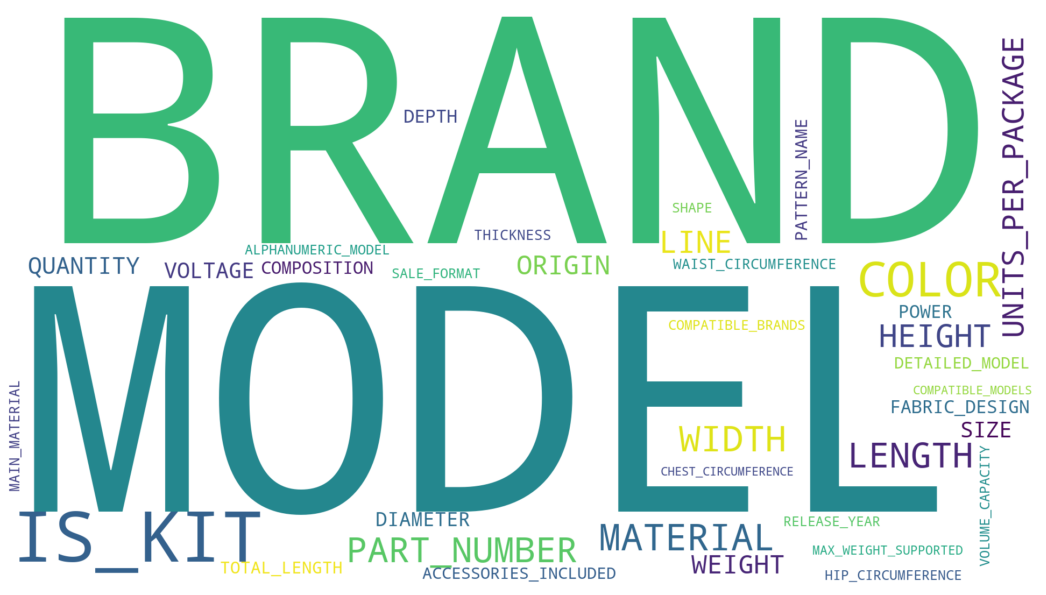
\includegraphics[width=0.80\linewidth]{atributos_em_numero_de_subcategorias.png}
	\caption{Nuvem de Palavras com os 39 atributos escolhidos para serem classes. O tamanho das palavras reflete o número de subcategorias do Mercado Livre em que esses atributos podem ser usados.}
	\label{fig:atributos_em_numero_de_subcategorias}
\end{figure}

Por outro lado, os atributos menos genéricos que foram definidos como classes, pois se encaixam nos critérios aplicados, são \textbf{CHEST\_CIRCUMFERENCE} e \textbf{COMPATIBLE\_MODELS}. Ambos os atributos podem ser usados em 87 subcategorias de produtos. \textbf{CHEST\_CIRCUMFERENCE}, traduzido como ``circunferência do busto'' em Português, se aplica apenas a itens de Vestuário, setor em que a empresa GoBots ainda não possui clientes, e por isso representa um bom experimento para avaliar a possibilidade de atração de clientes do setor. \textbf{COMPATIBLE\_MODELS}, de forma similar, é usado para descrever apenas a compatibilidade de peças e acessórios, como motores e válvulas, com modelos de objetos maiores, como veículos e eletrodomésticos. Portanto, o baixo número de subcategorias onde esses atributos podem ser usados se justifica pela especificidade de suas aplicações.

\section{Coleta de Dados}
\label{res:coleta_dados}
A Tabela \ref{table:coleta de dados} apresenta uma estimativa de qual porcentagem cada fonte de coleta de dados representa em relação a base de dados criada. A maior parte das perguntas, estimada em 70\%, foi coletada a partir do banco de dados da GoBots, que já existia anteriormente. Os outros 30\% foram coletados por meio de coleta manual no mercadolivre.com.br ou através de criação manual, em um esforço para garantir que cada classe possuísse pelo menos 15 exemplos. A coleta de dados através de criação manual foi de apenas 10\%, com o objetivo de fazer com que os exemplos vistos fossem, em sua grande maioria, representações da forma de perguntar de clientes reais. Em virtude do alto número de exemplos, não é possível saber com exatidão quantos exemplos foram coletados de cada fonte.

\begin{center}
\begin{table}[!ht]
\caption{Fontes para Coleta de Dados e estimativa de sua representatividade na base de dados}
\label{table:coleta de dados}
\centering
    \begin{tabular}{|c|c|} 
     \hline
     \multicolumn{2}{|c|}{Fonte dos Dados} \\
     \hline
     Banco de Dados da GoBots & 70\% \\ 
     \hline
     Coleta manual no mercadolivre.com.br & 20\% \\
     \hline
     Criação manual & 10\% \\
     \hline
     Total & 1419 \\
     \hline
    \end{tabular}
\end{table}
\end{center}

\section{Criação da Base de Dados Rotulada}
\label{res:criacao_base_dados_rotulada}
Como visto na Seção \ref{criacao_base_dados_rotulada}, a criação da base de dados rotulada ocorreu em duas rodadas. Na primeira rodada, as perguntas foram rotuladas em relação aos atributos a que elas se referem, considerando 40 atributos descritores de produtos do Mercado Livre. Na segunda rodada, atributos similares foram aglutinados em um único atributo, com o objetivo de minimizar a ocorrência de situações em que uma pergunta poderia ser classificada em mais de um atributo ao mesmo tempo. Isso proporcionou com que uma nova rotulação, baseada em 28 classes ao invés de 40, pudesse ser feita. 

A Tabela \ref{table:divisão_de_classes} apresenta a quantidade de exemplos rotulados para cada classe considerando a configuração inicialmente proposta na primeira rodada de experimentos, constituída de 40 classes:

\begin{table}[!htb]
\caption{Quantidade de exemplos rotulados para cada classe na configuração com 40 classes}
\label{table:divisão_de_classes}
\tiny % Define o tamanho da fonte para small (opcional)
\begin{tabularx}{\textwidth}{|X|c|X|c|}
 \hline
 \textbf{Classe} & \textbf{Exemplos} & \textbf{Classe} & \textbf{Exemplos} \\
 \hline
 BRAND & \textbf{105} & MODEL & \textbf{32} \\
 \hline
 IS\_KIT & \textbf{18} & COLOR & \textbf{94} \\
 \hline
 WIDTH & \textbf{32} & LENGTH & \textbf{29} \\
 \hline
 PART\_NUMBER & \textbf{21} & MATERIAL & \textbf{58} \\
 \hline
 HEIGHT & \textbf{41} & LINE & \textbf{23} \\
 \hline
 UNITS\_PER\_PACKAGE & \textbf{22} & ORIGIN & \textbf{25} \\
 \hline
 RELEASE\_YEAR & \textbf{27} & WEIGHT & \textbf{22} \\
 \hline
 QUANTITY & \textbf{23} & VOLTAGE & \textbf{60} \\
 \hline
 SIZE & \textbf{80} & DIAMETER & \textbf{26} \\
 \hline
 DEPTH & \textbf{21} & FABRIC\_DESIGN & \textbf{16} \\
 \hline
 POWER & \textbf{33} & COMPOSITION & \textbf{18} \\
 \hline
 PATTERN\_NAME & \textbf{16} & TOTAL\_LENGTH & \textbf{23} \\
 \hline
 DETAILED\_MODEL & \textbf{72} & ACCESSORIES\_INCLUDED & \textbf{55} \\
 \hline
 MAIN\_MATERIAL & \textbf{16} & THICKNESS & \textbf{29} \\
 \hline
 MATERIALS & \textbf{35} & WAIST\_CIRCUMFERENCE & \textbf{16} \\
 \hline
 VOLUME\_CAPACITY & \textbf{23} & HIP\_CIRCUMFERENCE & \textbf{15} \\
 \hline
 ALPHANUMERIC\_MODEL & \textbf{23} & COMPATIBLE\_BRANDS & \textbf{20} \\
 \hline
 SHAPE & \textbf{20} & SALE\_FORMAT & \textbf{34} \\
 \hline
 MAX\_WEIGHT\_SUPPORTED & \textbf{32} & CHEST\_CIRCUMFERENCE & \textbf{15} \\
 \hline
 COMPATIBLE\_MODELS & \textbf{48} & out\_of\_scope & \textbf{101} \\
 \hline
 \multicolumn{3}{|l|}{\textbf{Total de Exemplos}} & \textbf{1419} \\
 \hline
\end{tabularx}
\end{table}

É possível perceber o desbalanceamento entre o número de exemplos de cada classe. Esse desbalanceamento ocorreu, sobretudo, por conta da facilidade em se encontrar perguntas relacionadas a atributos como marca e cor do produto (perguntas classificadas como \textbf{BRAND} e \textbf{COLOR}) em detrimento da dificuldade de se encontrar perguntas relacionadas a atributos como a estampa de uma peça de roupa e os modelos compatíveis (perguntas classificadas como \textbf{FABRIC\_DESIGN} e \textbf{COMPATIBLE\_MODELS}). Essa dificuldade se justifica pelo menor número de subcategorias de produtos que podem receber esses atributos, como abordado na Seção \ref{res:definicao_classes}. A Figura \ref{fig:número_de_exemplos_40_classes} retrata, por meio de um gráfico de barras, o número de exemplos rotulados em cada classe.
% Gráfico de barras pras pessoas verem pelo tamanho das barras as classes com os maiores números de exemplos. É válido ter duas formas de representação gráfica pros mesmos dados.
% Gráfico de barras - 40 classes

\begin{figure}[!htb]
    \centering
	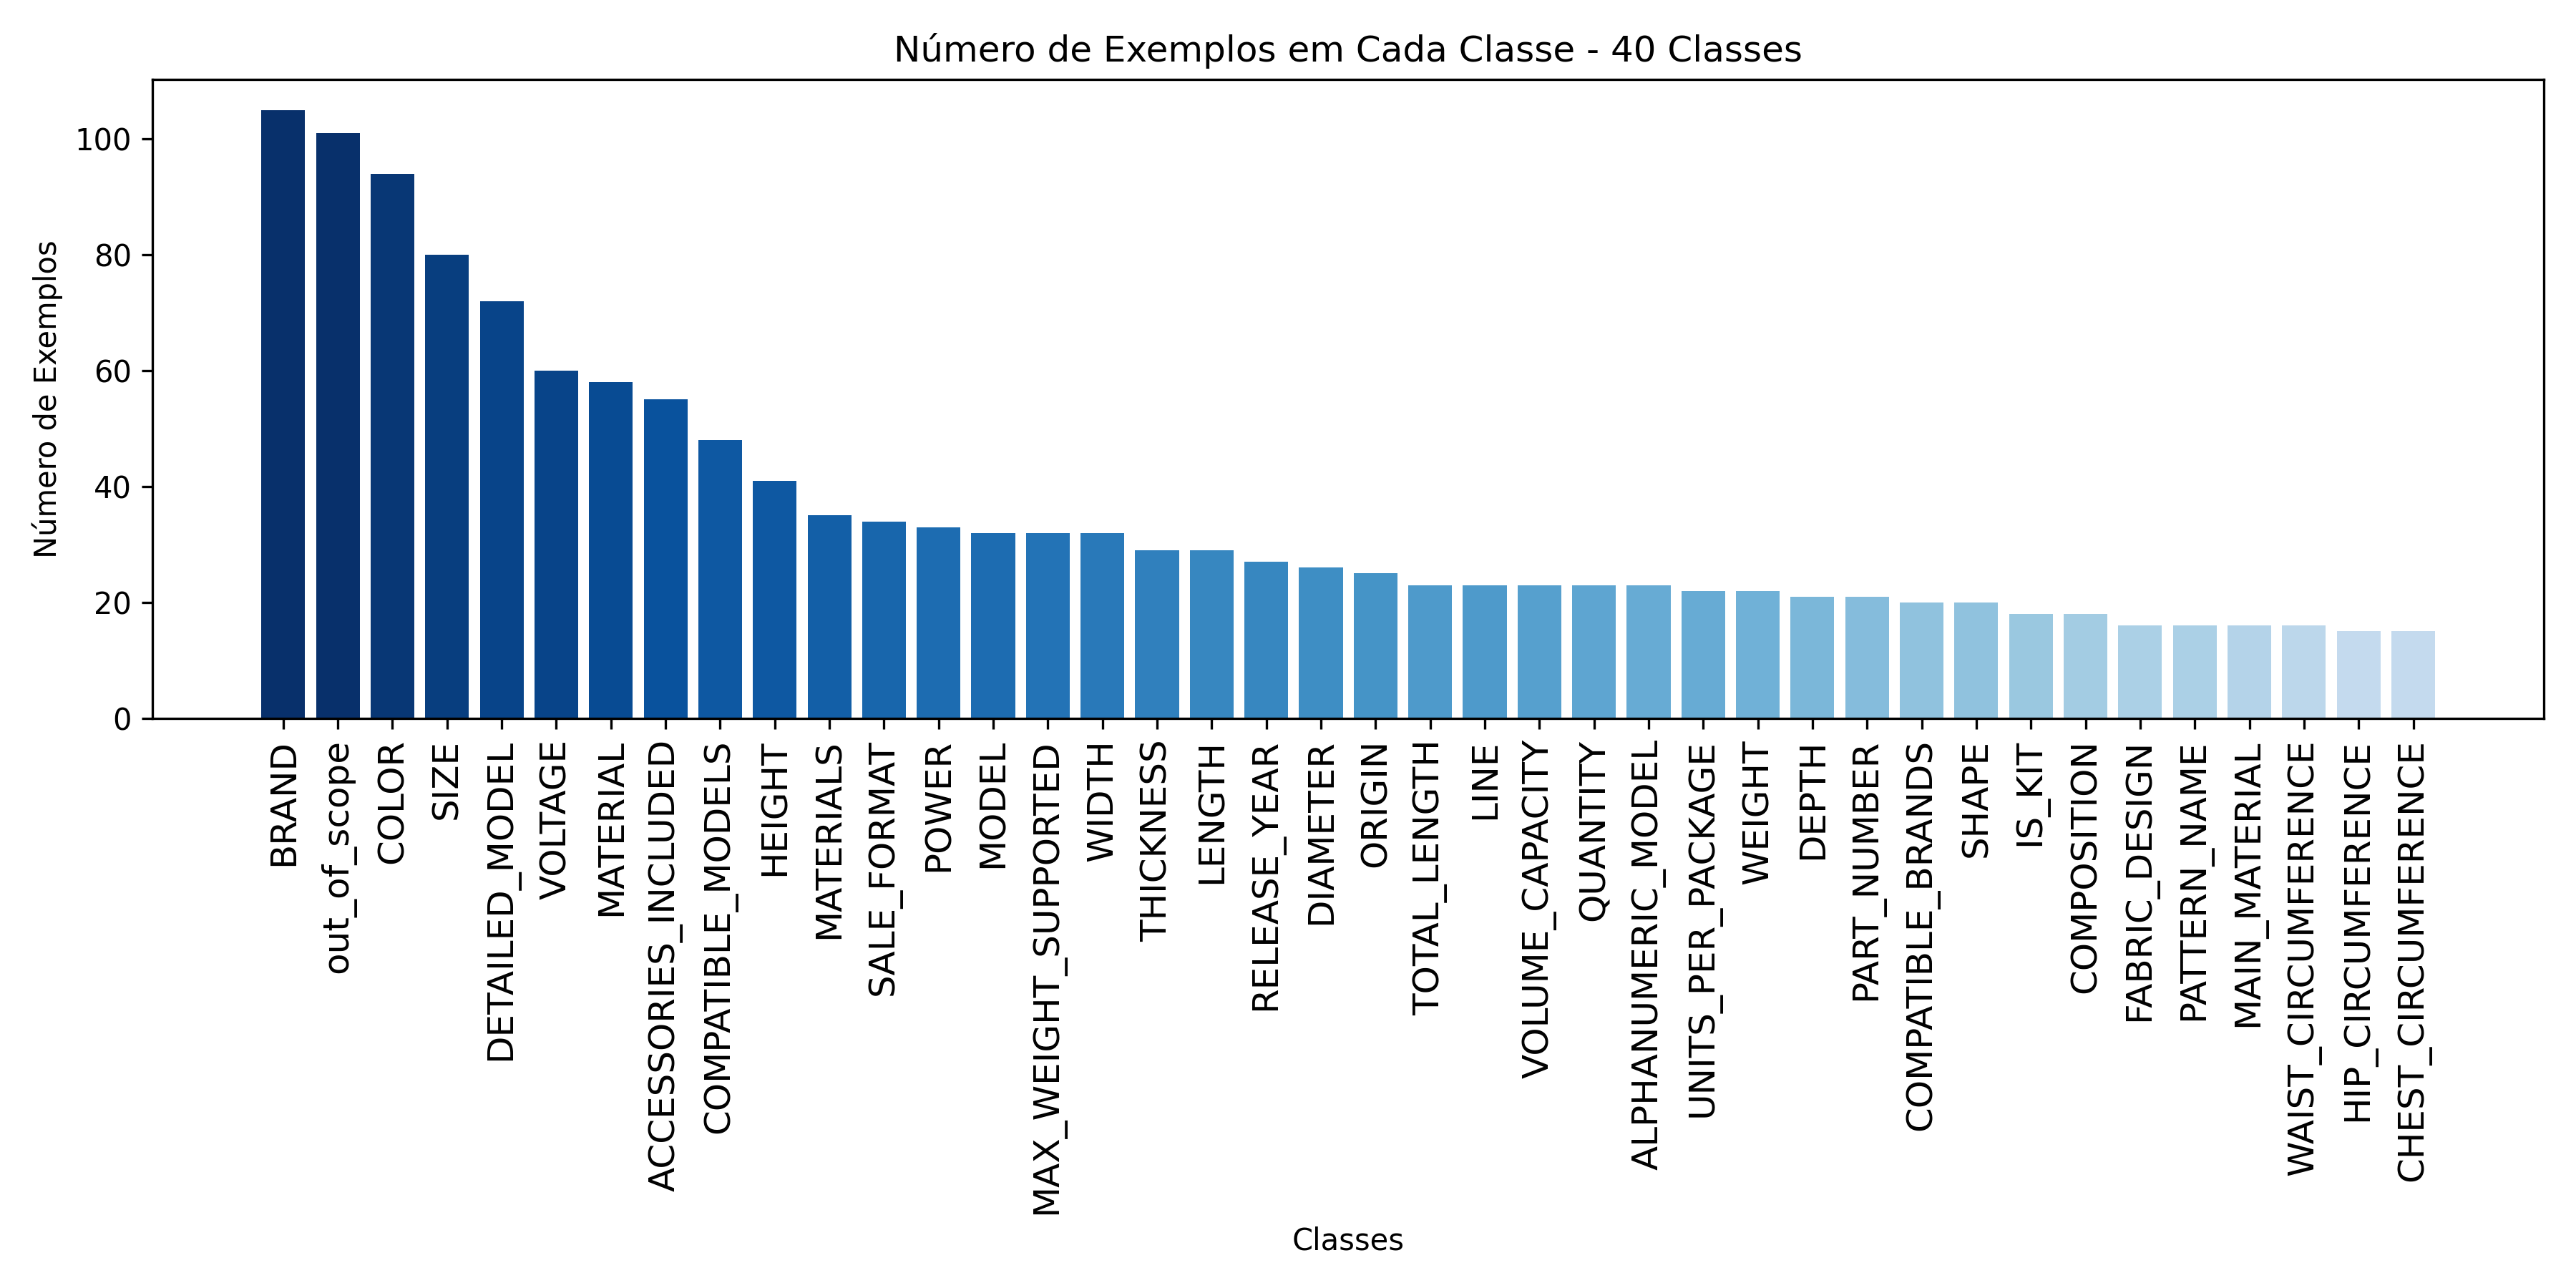
\includegraphics[width=1\linewidth]{figuras/número_de_exemplos_40_classes.png}
	\caption{Gráfico de Barras retratando o número total de exemplos rotulados para cada uma das 40 classes, da classe com mais exemplos para a com menos exemplos.}
	\label{fig:número_de_exemplos_40_classes}
\end{figure}

Para a segunda rodada de criação da base de dados rotulada, foi criada uma nova base de dados, com 28 classes. A quantidade de exemplos de cada classe está descrita na Tabela \ref{table:nova_divisão_de_classes} e as aglutinações de classes feitas foram ilustradas na Figura \ref{fig:aglutinacao_classes}. 

\begin{table}[!ht]
\caption{Quantidade de exemplos rotulados para cada classe na configuração com 28 classes}
\label{table:nova_divisão_de_classes}
\tiny % Define o tamanho da fonte para small (opcional)
\begin{tabularx}{\textwidth}{|X|c|X|c|}
 \hline
 \textbf{Classe} & \textbf{Exemplos} & \textbf{Classe} & \textbf{Exemplos} \\
 \hline
 BRAND & \textbf{105} & MODEL & \textbf{127} \\
 \hline
 COLOR & \textbf{94} & PART\_NUMBER & \textbf{21} \\
 \hline
 MATERIAL & \textbf{127} & LINE & \textbf{23} \\
 \hline
 ORIGIN & \textbf{25} & RELEASE\_YEAR & \textbf{27} \\
 \hline
 WEIGHT & \textbf{22} & QUANTITY & \textbf{97} \\
 \hline
 VOLTAGE & \textbf{60} & SIZE & \textbf{205} \\
 \hline
 DIAMETER & \textbf{26} & DEPTH & \textbf{21} \\
 \hline
 FABRIC\_DESIGN & \textbf{16} & POWER & \textbf{33} \\
 \hline
 PATTERN\_NAME & \textbf{16} & ACCESSORIES\_INCLUDED & \textbf{55} \\
 \hline
 THICKNESS & \textbf{29} & WAIST\_CIRCUMFERENCE & \textbf{16} \\
 \hline
 VOLUME\_CAPACITY & \textbf{23} & HIP\_CIRCUMFERENCE & \textbf{15} \\
 \hline
 COMPATIBLE\_BRANDS & \textbf{20} & SHAPE & \textbf{20} \\
 \hline
 MAX\_WEIGHT\_SUPPORTED & \textbf{32} & CHEST\_CIRCUMFERENCE & \textbf{15} \\
 \hline
 COMPATIBLE\_MODELS & \textbf{48} & out\_of\_scope & \textbf{101} \\
 \hline
 \multicolumn{3}{|l|}{\textbf{Total de Exemplos}} & \textbf{1419} \\
 \hline
\end{tabularx}
\end{table}
% Gráfico de barras - 28 classes
% Criação da Base Rotulada: nuvem de palavras sobre os atributos (classes) com o maior número de exemplos. É uma boa para mostrar o desbalanceamento da base de dados.

A partir da Tabela \ref{table:nova_divisão_de_classes}, é possível perceber que o problema de desbalanceamento de classes se acentuou ainda mais por causa da aglutinação. Isso pode ocasionar um efeito negativo nas métricas de avaliação e será analisado nas seções posteriores. Contudo, o objetivo principal de minimizar a ocorrência de situações em que uma pergunta poderia ser classificada em mais de um atributo ao mesmo tempo foi atingido. Além disso, nenhum exemplo foi removido da base de dados. A Figura \ref{fig:número_de_exemplos_28_classes} retrata, por meio de um gráfico de barras, o número de exemplos rotulados em cada classe nessa configuração com 28 classes.

\begin{figure}[!htb]
    \centering
	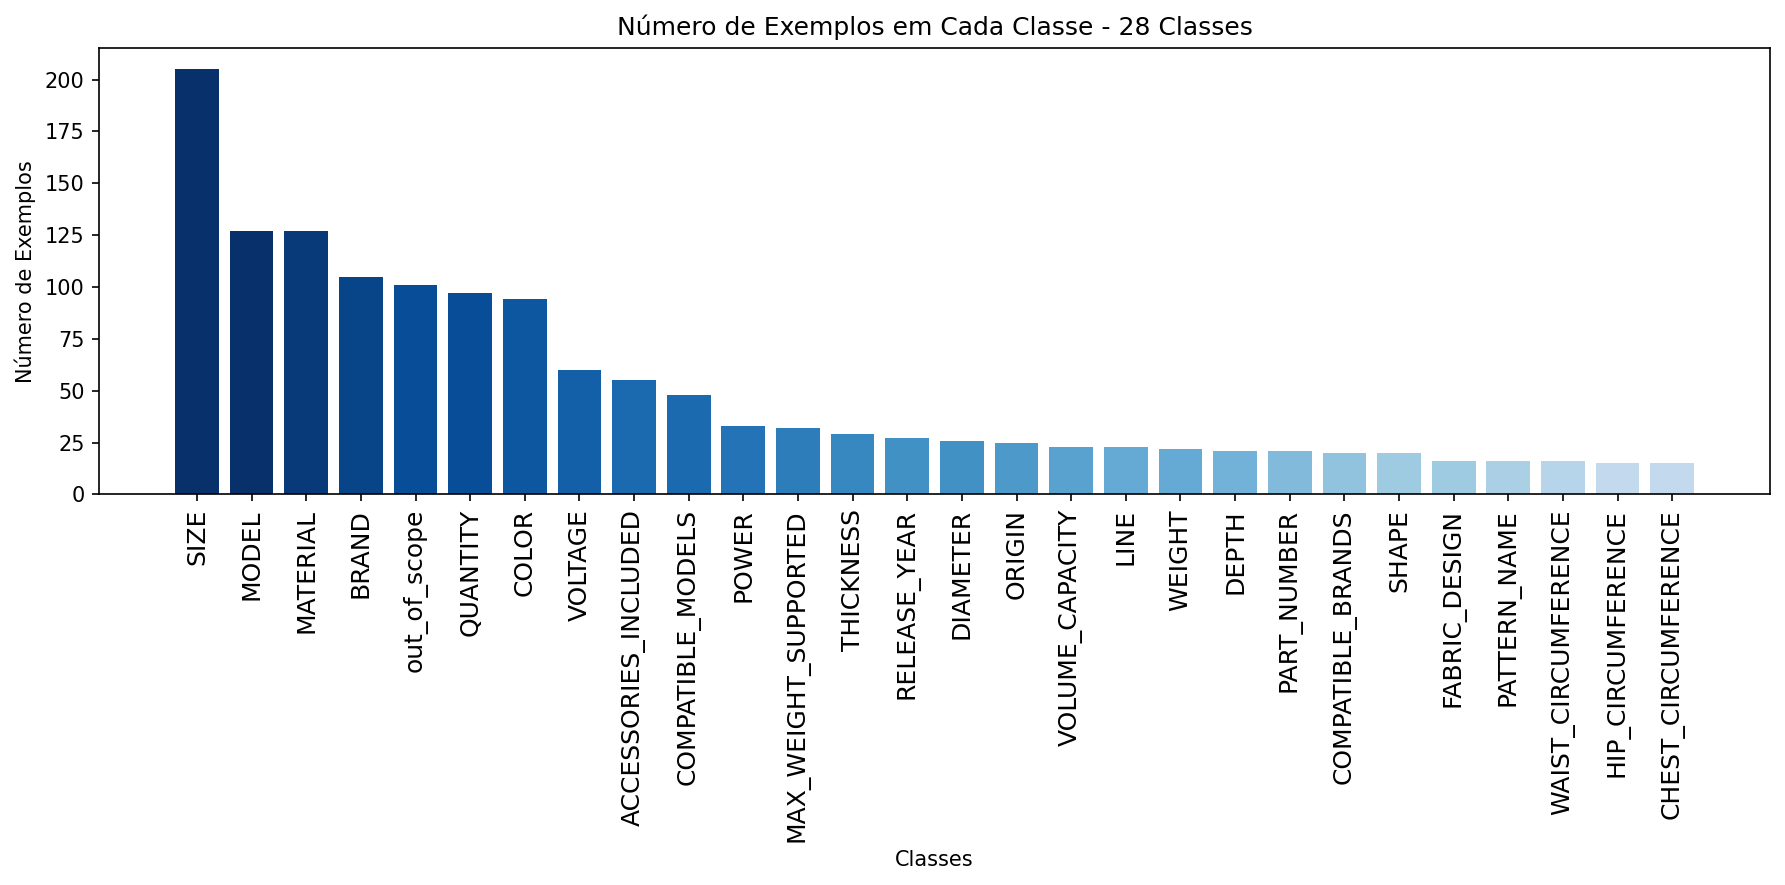
\includegraphics[width=1\linewidth]{figuras/número_de_exemplos_28_classes.png}
	\caption{Gráfico de Barras retratando o número total de exemplos rotulados para cada uma das 28 classes, da classe com mais exemplos para a com menos exemplos.}
	\label{fig:número_de_exemplos_28_classes}
\end{figure}

Analisando a Figura \ref{fig:número_de_exemplos_28_classes}, é possível perceber que \textbf{SIZE} (tamanho) passou a ser a classe com o maior número de exemplos. \textbf{BRAND} (marca), que na primeira rodada da criação da base de dados rotulada era a classe com o maior número de exemplos, passou a ser apenas a 4\textsuperscript{a} maior classe. Outras classes resultantes de aglutinação, \textbf{MODEL} (modelo), \textbf{MATERIAL} (material), e \textbf{QUANTITY} (quantidade), passaram a ser a 2\textsuperscript{a}, 3\textsuperscript{a}, e 6\textsuperscript{a} maior classe, respectivamente. Pelo fato de possuírem um maior número de exemplos quando considerando a base de dados com 28 classes, espera-se que as medidas de avaliação dos modelos classificadores nessas classes aglutinadas sejam melhoradas.


\section{Treinamento e Avaliação dos Classificadores}
\label{res:treinamento_avaliacao_dos_classificadores}
A seguir, será apresentada uma discussão quanto ao desempenho individual de cada um dos algoritmos de classificação treinados, em cada uma das configurações apresentadas. Em um primeiro momento, serão apresentados os resultados dos experimentos envolvendo a base de dados com 40 classes. Em seguida, serão apresentados os resultados dos experimentos envolvendo a base de dados com classes aglutinadas, de 28 classes. 

\subsection{Configuração do Treinamento e Método de Avaliação}
A Tabela \ref{table:divisão_de_classes_com_validação} mostra o número de exemplos de Treino e Teste em cada classe na primeira rodada de experimentos, de 40 classes, enquanto a Tabela \ref{table:nova_divisão_de_classes_com_validação} mostra o número de exemplos de Treino e Teste em cada classe na segunda rodada de experimentos, de 28 classes.

\begin{table}[ht]
\caption{Quantidade de exemplos de Treino e Teste para cada classe na configuração com 40 classes}
\label{table:divisão_de_classes_com_validação}
\tiny % Define o tamanho da fonte para small (opcional)
\begin{tabularx}{\textwidth}{|X|c|c|c|} 
 \hline
 \textbf{Classe} & \textbf{Exemplos de Treino} & \textbf{Exemplos de Teste} & \textbf{Total de Exemplos} \\
 \hline
 BRAND & 84 & 21 & \textbf{105}\\
 \hline
 MODEL & 26 & 6 & \textbf{32}\\
 \hline
 IS\_KIT & 14 & 4 & \textbf{18}\\
 \hline
 COLOR & 75 & 19 & \textbf{94}\\
 \hline
 WIDTH & 25 & 7 & \textbf{32}\\
 \hline
 LENGTH & 23 & 6 & \textbf{29}\\
 \hline
 PART\_NUMBER & 16 & 5 & \textbf{21}\\
 \hline
 MATERIAL & 46 & 12 & \textbf{58}\\
 \hline
 HEIGHT & 32 & 9 & \textbf{41}\\
 \hline
 LINE & 19 & 4 & \textbf{23}\\
 \hline
 UNITS\_PER\_PACKAGE & 18 & 4 & \textbf{22}\\
 \hline
 ORIGIN & 20 & 5 & \textbf{25}\\
 \hline
 RELEASE\_YEAR & 22 & 5 & \textbf{27}\\
 \hline
 WEIGHT & 17 & 5 & \textbf{22}\\
 \hline
 QUANTITY & 18 & 5 & \textbf{23}\\
 \hline
 VOLTAGE & 48 & 12 & \textbf{60}\\
 \hline
 SIZE & 64 & 16 & \textbf{80}\\
 \hline
 DIAMETER & 21 & 5 & \textbf{26}\\
 \hline
 DEPTH & 17 & 4 & \textbf{21}\\
 \hline
 FABRIC\_DESIGN & 12 & 4 & \textbf{16}\\
 \hline
 POWER & 26 & 7 & \textbf{33}\\
 \hline
 COMPOSITION & 15 & 3 & \textbf{18}\\
 \hline
 PATTERN\_NAME & 13 & 3 & \textbf{16}\\
 \hline
 TOTAL\_LENGTH & 19 & 4 & \textbf{23}\\
 \hline
 DETAILED\_MODEL & 58 & 14 & \textbf{72}\\
 \hline
 ACCESSORIES\_INCLUDED & 44 & 11 & \textbf{55}\\
 \hline
 MAIN\_MATERIAL & 13 & 3 & \textbf{16}\\
 \hline
 THICKNESS & 23 & 6 & \textbf{29}\\
 \hline
 MATERIALS & 28 & 7 & \textbf{35}\\
 \hline
 WAIST\_CIRCUMFERENCE & 13 & 3 & \textbf{16}\\
 \hline
 VOLUME\_CAPACITY & 18 & 5 & \textbf{23}\\
 \hline
 HIP\_CIRCUMFERENCE & 12 & 3 & \textbf{15}\\
 \hline
 ALPHANUMERIC\_MODEL & 18 & 5 & \textbf{23}\\
 \hline
 COMPATIBLE\_BRANDS & 16 & 4 & \textbf{20}\\
 \hline
 SHAPE & 16 & 4 & \textbf{20}\\
 \hline
 SALE\_FORMAT & 28 & 6 & \textbf{34}\\
 \hline
 MAX\_WEIGHT\_SUPPORTED & 26 & 6 & \textbf{32}\\
 \hline
 CHEST\_CIRCUMFERENCE & 12 & 3 & \textbf{15}\\
 \hline
 COMPATIBLE\_MODELS & 39 & 9 & \textbf{48}\\
 \hline
 out\_of\_scope & 81 & 20 & \textbf{101}\\
 \hline
 \textbf{Total} & \textbf{1135} & \textbf{284} & \textbf{1419}\\
 \hline
\end{tabularx}
\end{table}

\begin{table}[H]
\caption{Quantidade de exemplos de Treino e Teste para cada classe na configuração com 28 classes}
\label{table:nova_divisão_de_classes_com_validação}
\tiny % Define o tamanho da fonte para small (opcional)
\begin{tabularx}{\textwidth}{|X|c|c|c|} 
 \hline
 \textbf{Classe} & \textbf{Exemplos de Treino} & \textbf{Exemplos de Teste} & \textbf{Total de Exemplos} \\
 \hline
 BRAND & 84 & 21 & \textbf{105}\\
 \hline
 MODEL & 102 & 25 & \textbf{127}\\
 \hline
 COLOR & 75 & 19 & \textbf{94}\\
 \hline
 PART\_NUMBER & 16 & 5 & \textbf{21}\\
 \hline
 MATERIAL & 102 & 25 & \textbf{127}\\
 \hline
 LINE & 19 & 4 & \textbf{23}\\
 \hline
 ORIGIN & 20 & 5 & \textbf{25}\\
 \hline
 RELEASE\_YEAR & 22 & 5 & \textbf{27}\\
 \hline
 WEIGHT & 17 & 5 & \textbf{22}\\
 \hline
 QUANTITY & 78 & 19 & \textbf{97}\\
 \hline
 VOLTAGE & 48 & 12 & \textbf{60}\\
 \hline
 SIZE & 163 & 42 & \textbf{205}\\
 \hline
 DIAMETER & 21 & 5 & \textbf{26}\\
 \hline
 DEPTH & 17 & 4 & \textbf{21}\\
 \hline
 FABRIC\_DESIGN & 12 & 4 & \textbf{16}\\
 \hline
 POWER & 26 & 7 & \textbf{33}\\
 \hline
 PATTERN\_NAME & 13 & 3 & \textbf{16}\\
 \hline
 ACCESSORIES\_INCLUDED & 44 & 11 & \textbf{55}\\
 \hline
 THICKNESS & 23 & 6 & \textbf{29}\\
 \hline
 WAIST\_CIRCUMFERENCE & 13 & 3 & \textbf{16}\\
 \hline
 VOLUME\_CAPACITY & 18 & 5 & \textbf{23}\\
 \hline
 HIP\_CIRCUMFERENCE & 12 & 3 & \textbf{15}\\
 \hline
 COMPATIBLE\_BRANDS & 16 & 4 & \textbf{20}\\
 \hline
 SHAPE & 16 & 4 & \textbf{20}\\
 \hline
 MAX\_WEIGHT\_SUPPORTED & 26 & 6 & \textbf{32}\\
 \hline
 CHEST\_CIRCUMFERENCE & 12 & 3 & \textbf{15}\\
 \hline
 COMPATIBLE\_MODELS & 39 & 9 & \textbf{48}\\
 \hline
 out\_of\_scope & 81 & 20 & \textbf{101}\\
 \hline
 \textbf{Total} & \textbf{1135} & \textbf{284} & \textbf{1419}\\
 \hline
\end{tabularx}
\end{table}


\subsection{Experimentos com 40 Classes}
\label{res:experimentos_40classes}
As Tabelas \ref{tab:metricas_maximas_40classes} e \ref{tab:metricas_gerais_40classes} apresentam os resultados da primeira rodada de experimentos, que usou a base de dados com 40 classes. A Tabela \ref{tab:metricas_maximas_40classes} mostra o número de classes que atingiram o valor máximo de Revocação e Precisão, assim como o número de classes que atingiram o valor mínimo dessas métricas. A Tabela \ref{tab:metricas_gerais_40classes} traz um sumário das métricas de avaliação de cada modelo ponderadas pelo número de exemplos em cada classe. Os modelos estão identificados com os nomes definidos nas Seções \ref{des_treinamento_hf} e \ref{des_treinamento_rasa}. As Matrizes de Confusão estão dispostas no Apêndice \ref{ap:matrizes_de_confusao}.

É possível perceber pela Tabela \ref{tab:metricas_maximas_40classes} que o modelo no qual mais classes tiveram todos os seus exemplos corretamente previstos foi o modelo HF2. Ao mesmo tempo, esse modelo se destacou negativamente pelo fato de não ter previsto corretamente nenhum exemplo de 6 classes, o que indica que o modelo confunde essas classes com outras classes que apresentam exemplos similares.

O modelo que apresentou nos testes o maior número de classes com Precisão igual a 1 foi o modelo HF1. Esse resultado indica que é possível ter grande confiança nesse modelo quando ele prevê que uma pergunta é de determinada classe, ao menos para as classes que apresentaram o valor máximo de Precisão.

Ao prever corretamente ao menos 1 exemplo de Teste para todas as classes, o modelo RASA1 se mostrou um modelo generalista, ou seja, com habilidade de aprender características de todas as classes. Os outros modelos que possuem como algoritmo de classificação o modelo DIETClassifier apresentaram resultados próximos.

\begin{table}[!ht]
\centering
\caption{Número de classes que atingiram o valor máximo e o valor mínimo das métricas de avaliação (base de dados com 40 classes)}
\label{tab:metricas_maximas_40classes}
\resizebox{\textwidth}{!}{%
\begin{tabular}{|c|c|c|c|c|}
\hline
\textbf{ID} & \textbf{Revocação = 1} & \textbf{Precisão = 1} & \textbf{Revocação = 0 e Precisão = 0} \\
\hline
HF1 & 10 & \textbf{16} & 4 \\
\hline
HF2 & \textbf{16} & 13 & 6 \\
\hline 
RASA1 & 10 & 12 & \textbf{0} \\
\hline
RASA2 & 9 & 14 & 1 \\
\hline
RASA3 & 12 & 12 & 1 \\
\hline
\end{tabular}
}
\end{table}

A Tabela \ref{tab:metricas_gerais_40classes} mostra que o modelo HF2 obteve os melhores resultados gerais, apesar do grande número de classes em que nenhum exemplo foi corretamente previsto. Os resultados mostram que esse modelo se mostrou um modelo especialista em algumas classes. Por esse motivo, ele foi o modelo BERT escolhido para os experimentos com a base de dados aglutinada. O modelo RASA3 se destacou em relação à Precisão e por isso foi o modelo DIETClassifier escolhido. 

\begin{table}[!ht]
\centering
\caption{Métricas de avaliação ponderadas pelo número de exemplos de cada classe (base de dados com 40 classes)}
\label{tab:metricas_gerais_40classes}
\resizebox{\textwidth}{!}{%
\begin{tabular}{|c|c|c|c|c|c|c|}
\hline
\textbf{ID} & \textbf{Encoder} & \textbf{Classificador} & \textbf{Acurácia} & \textbf{F1-Score} & \textbf{Precisão} & \textbf{Revocação} \\
\hline
HF1 & BERTimbau & BERTimbau & 0,702 & 0,669 & 0,686 & 0,702 \\
\hline
HF2 & BERTimbau & BERTimbau & \textbf{0,749} & \textbf{0,720} & 0,720 & \textbf{0,749} \\
\hline
RASA1 & BERT-Multi & DIET & 0,680 & 0,668 & 0,705 & 0,680 \\
\hline
RASA2 & BERTimbau & DIET & 0,687 & 0,673 & 0,700 & 0,687 \\
\hline
RASA3 & BERTimbau & DIET & 0,718 & 0,711 & \textbf{0,731} & 0,718 \\
\hline
\end{tabular}}
\end{table}

A Tabela \ref{tab:melhores_classes_revocação_40_classes} sumariza as classes que obtiveram os melhores desempenhos na medida Revocação. Todas as classes mostradas obtiveram desempenho máximo, ou seja, todos os seus exemplos de Teste foram corretamente classificados. Uma característica em comum entre essas classes é que seus exemplos são compostos por palavras ou termos frequentemente repetidos, o que facilita a predição.

\begin{table}[!ht]
\centering
\caption{Classes com os maiores valores de Revocação (base de dados com 40 classes)}
\label{tab:melhores_classes_revocação_40_classes}
\resizebox{\textwidth}{!}{%
\begin{tabular}{|c|c|c|c|c|c|c|c|}
\hline
\textbf{Posição} & \textbf{Classe} & \textbf{HF1} & \textbf{HF2} & \textbf{RASA1} & \textbf{RASA2} & \textbf{RASA3} & \textbf{Média} \\
\hline
1° & DEPTH & 1,000 & 1,000 & 1,000 & 1,000 & 1,000 & 1,000 \\
\hline
1° & HIP\_CIRCUMFERENCE & 1,000 & 1,000 & 1,000 & 1,000 & 1,000 & 1,000 \\
\hline
1° & THICKNESS & 1,000 & 1,000 & 1,000 & 1,000 & 1,000 & 1,000 \\
\hline
1° & VOLTAGE & 1,000 & 1,000 & 1,000 & 1,000 & 1,000 & 1,000 \\
\hline
1° & VOLUME\_CAPACITY & 1,000 & 1,000 & 1,000 & 1,000 & 1,000 & 1,000 \\
\hline
1° & WAIST\_CIRCUNFERENCE & 1,000 & 1,000 & 1,000 & 1,000 & 1,000 & 1,000 \\
\hline
\end{tabular}}
\end{table}

A Tabela \ref{tab:piores_classes_revocação_40_classes} sumariza as classes que obtiveram os piores desempenhos na medida Revocação, ou seja, as classes em que percentualmente menos exemplos de Teste foram classificados corretamente. É possível perceber que 4 das 5 classes apresentadas são compostas de exemplos que poderiam ser classificados em mais de uma classe ao mesmo tempo na ausência de informações complementares, situação que o procedimento de aglutinação de classes tenta resolver. \textbf{COMPATIBLE\_BRANDS}, no entanto, representa um problema maior: ela é uma classe que foi confundida com \textbf{COMPATIBLE\_MODELS} em 4 dos 5 modelos, e um modelo necessitaria de conhecimento de mundo para poder classificá-la corretamente.

\begin{table}[!ht]
\centering
\caption{Classes com os piores valores de Revocação (base de dados com 40 classes)}
\label{tab:piores_classes_revocação_40_classes}
\resizebox{\textwidth}{!}{%
\begin{tabular}{|c|c|c|c|c|c|c|c|}
\hline
\textbf{Posição} & \textbf{Classe} & \textbf{HF1} & \textbf{HF2} & \textbf{RASA1} & \textbf{RASA2} & \textbf{RASA3} & \textbf{Média} \\
\hline
40° & COMPATIBLE\_BRANDS & 0,0000 & 0,0000 & 0,5000 & 0,0000 & 0,0000 & 0,1000 \\
\hline
39° & ALPHANUMERIC\_MODEL & 0,0000 & 0,0000 & 0,2000 & 0,2000 & 0,6000 & 0,2000 \\
\hline
38° & UNITS\_PER\_PACKAGE & 0,0000 & 0,0000 & 0,2500 & 0,5000 & 0,5000 & 0,2500 \\
\hline
37° & MATERIALS & 0,1429 & 0,0000 & 0,5714 & 0,4286 & 0,5714 & 0,3429 \\
\hline
36° & MODEL & 0,1667 & 0,3333 & 0,6667 & 0,1667 & 0,5000 & 0,3667 \\
\hline
\end{tabular}}
\end{table}

\subsection{Experimentos com 28 Classes}
As Tabelas \ref{tab:metricas_maximas_28classes} e \ref{tab:metricas_gerais_28classes} apresentam o desempenho dos modelos treinados na base de dados com 28 classes e aglutinações de classes propostas na Seção \ref{criacao_base_dados_rotulada}. Os modelos treinados nessa etapa são iguais aos modelos treinados na etapa anterior. As Matrizes de Confusão estão dispostas no Apêndice \ref{ap:matrizes_de_confusao}.

O resultado mostrado na Tabela \ref{tab:metricas_maximas_28classes} indica que nesse cenário o modelo HF2 performou melhor que o modelo RASA3 em todos os aspectos. A diminuição no número de classes em que os modelos atingiram o valor máximo das métricas de avaliação é naturalmente esperada pela aplicação da aglutinação de classes. O modelo RASA3 apresentou dificuldade em aprender quando classificar um exemplo como \textbf{MODEL}: os exemplos dessa classe foram classificados como pertencentes a 10 classes diferentes.

\begin{table}[!ht]
\centering
\caption{Número de classes que atingiram o valor máximo e o valor mínimo das métricas de avaliação (base de dados com 28 classes)}
\label{tab:metricas_maximas_28classes}
\resizebox{\textwidth}{!}{%
\begin{tabular}{|c|c|c|c|c|}
\hline
\textbf{ID} & \textbf{Revocação = 1} & \textbf{Precisão = 1} & \textbf{Revocação = 0 e Precisão = 0} \\
\hline
HF2 & \textbf{11} & \textbf{11} & \textbf{1} \\
\hline 
RASA3 & \textbf{11} & 7 & \textbf{1} \\
\hline
\end{tabular}
}
\end{table}

A Tabela \ref{tab:metricas_gerais_28classes} confirma o bom desempenho do modelo HF2 quando comparado ao modelo RASA3. Além disso, ela demonstra que a aplicação da aglutinação de classes foi benéfica para os modelos: houve uma melhoria de 14,8\% em Acurácia, de 18,6\% em F1-Score, de 19,7\% em Precisão e de 14,8\% em Revocação no desempenho do modelo HF2 na base de dados com 28 classes em comparação ao desempenho do modelo HF2 na base de dados com 40 classes. O modelo RASA3 também foi influenciado positivamente pelo procedimento, porém com menos intensidade.

\begin{table}[!ht]
\centering
\caption{Métricas de avaliação ponderadas pelo número de exemplos de cada classe (base de dados com 28 classes)}
\label{tab:metricas_gerais_28classes}
\resizebox{\textwidth}{!}{%
\begin{tabular}{|c|c|c|c|c|c|c|}
\hline
\textbf{ID} & \textbf{Encoder} & \textbf{Classificador} & \textbf{Acurácia} & \textbf{F1-Score} & \textbf{Precisão} & \textbf{Revocação} \\
\hline
HF2 & BERTimbau & BERTimbau & \textbf{0,860} & \textbf{0,854} & \textbf{0,862} & \textbf{0,860} \\
\hline
RASA3 & BERTimbau & DIET & 0,763 & 0,755 & 0,775 & 0,763 \\
\hline
\end{tabular}}
\end{table}

A Tabela \ref{tab:melhores_classes_revocação_28_classes} sumariza as classes da base de dados com 28 classes que obtiveram os melhores desempenhos na medida Revocação, ou seja, as classes em que percentualmente mais exemplos de Teste foram classificados corretamente. Mais uma vez, há predomínio de classes consideradas de fácil predição, com exceção de \textbf{ORIGIN}.

\begin{table}[!ht]
\centering
\caption{Classes com os maiores valores de Revocação (base de dados com 28 classes)}
\label{tab:melhores_classes_revocação_28_classes}
\begin{tabular}{|c|c|c|c|c|}
\hline
\textbf{Posição} & \textbf{Classe} & \textbf{HF2} & \textbf{RASA3} & \textbf{Média} \\
\hline
1° & CHEST\_CIRCUMFERENCE & 1,000 & 1,000 & 1,000 \\
\hline
1° & DEPTH & 1,000 & 1,000 & 1,000 \\
\hline
1° & DIAMETER & 1,000 & 1,000 & 1,000 \\
\hline
1° & HIP\_CIRCUMFERENCE & 1,000 & 1,000 & 1,000 \\
\hline
1° & ORIGIN & 1,000 & 1,000 & 1,000 \\
\hline
1° & WAIST\_CIRCUNFERENCE & 1,000 & 1,000 & 1,000 \\
\hline
1° & WEIGHT & 1,000 & 1,000 & 1,000 \\
\hline
\end{tabular}
\end{table}

A Tabela \ref{tab:piores_classes_revocação_28_classes} sumariza as classes que obtiveram os piores desempenhos na medida Revocação. No geral, os modelos apresentaram valores mais altos para essa métrica do que os valores vistos na Tabela \ref{tab:piores_classes_revocação_40_classes}, o que confirma a eficácia da aglutinação de classes. A classe \textbf{MODEL} foi a única entre as classes aglutinadas que continuou na lista das 5 classes com os piores resultados.

A classe \textbf{COMPATIBLE\_BRANDS}, que havia sido a classe com os piores resultados na etapa anterior, continuou a ser a classe em que os modelos mais apresentam dificuldade de predição. A média de pontuação em Revocação era de 0,1000 no experimento anterior. No experimento com 28 classes, essa média caiu para 0,0000. Isso indica que nenhum dos dois modelos que tiveram os melhores desempenhos foi capaz de classificar corretamente 1 pergunta como \textbf{COMPATIBLE\_BRANDS}.

De forma geral, não é possível apontar um modelo mais generalista e um modelo mais especialista entre os modelos treinados na base de dados de 28 classes. Ambos os modelos não conseguiram prever corretamente os exemplos de uma única classe. Sendo assim, como as medidas de avaliação do modelo HF2 descritas na Tabela \ref{tab:metricas_gerais_28classes} apontam um desempenho geral muito superior desse modelo, ele é o melhor modelo treinado considerando as duas rodadas de experimentos.

\begin{table}[!ht]
\centering
\caption{Classes com os piores valores de Revocação (base de dados com 28 classes)}
\label{tab:piores_classes_revocação_28_classes}
\begin{tabular}{|c|c|c|c|c|}
\hline
\textbf{Posição} & \textbf{Classe} & \textbf{HF2} & \textbf{RASA3} & \textbf{Média} \\
\hline
28° & COMPATIBLE\_BRANDS & 0,000 & 0,000 & 0,000 \\
\hline
27° & MAX\_WEIGHT\_SUPPORTED & 0,500 & 0,500 & 0,500 \\
\hline
27° & SHAPE & 0,250 & 0,750 & 0,500 \\
\hline
25° & MODEL & 0,720 & 0,320 & 0,520 \\
\hline
24° & COMPATIBLE\_MODELS & 0,667 & 0,556 & 0,611 \\
\hline
\end{tabular}
\end{table}

\section{Comparativo entre Classes Frequentemente Confundidas}
\label{res:comparativo_entre_classes_confundidas}
As Figuras \ref{fig:compatible_brands} e \ref{fig:compatible_models} apresentam as nuvens de palavras geradas a partir dos exemplos de Treino e de Teste das classes \textbf{COMPATIBLE\_BRANDS} e \textbf{COMPATIBLE\_MODELS}, respectivamente.

É possível perceber que, apesar dessas duas classes serem frequentemente confundidas, as palavras que compõem seus exemplos se repetem pouco entre si. A maior exceção está relacionada à palavra \textbf{compatível}, que aparece 9 vezes nos exemplos da classe \textbf{COMPATIBLE\_BRANDS} e 16 vezes nos exemplos da classe \textbf{COMPATIBLE\_MODELS}.

É possível concluir que um dos motivos para a dificuldade apresentada pelos modelos em classificar corretamente os exemplos da classe \textbf{COMPATIBLE\_BRANDS} é a falta de conhecimento de mundo para entender quais palavras representam marcas e quais palavras representam modelos. Como estatisticamente a palvra \textbf{compatível} aparece mais vezes na classe \textbf{COMPATIBLE\_MODELS}, os modelos esperam que qualquer exemplo que apresente essa palavra também pertença a essa classe. Uma possível solução para esse problema é fazer uso de grandes estruturas de dados que salvem nomes de marcas e de modelos, como o grafo de conhecimento interno do Mercado Livre. Uma solução alternativa que poderia ser testada é o uso de outros modelos de Aprendizado Profundo que possuam um maior número de parâmetros.

\begin{figure}[!ht]
    \centering
	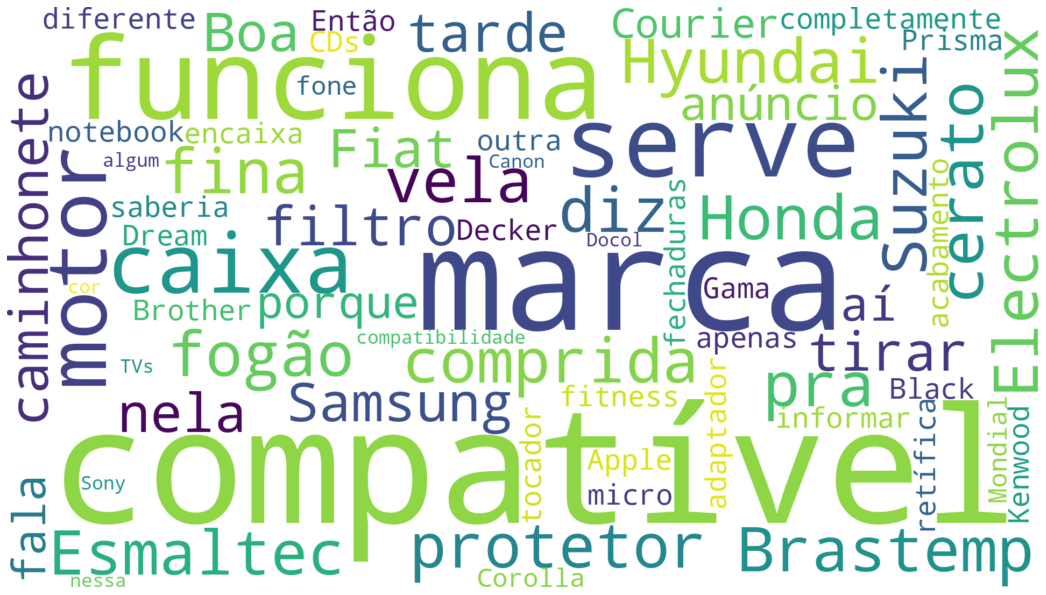
\includegraphics[width=1\linewidth]{figuras/compatible_brands.png}
	\caption{Nuvem de palavras gerada a partir dos exemplos de Treino e Teste da classe \textbf{COMPATIBLE\_BRANDS}, após remoção de \textit{stopwords}.}
	\label{fig:compatible_brands}
\end{figure}

\begin{figure}[!ht]
    \centering
	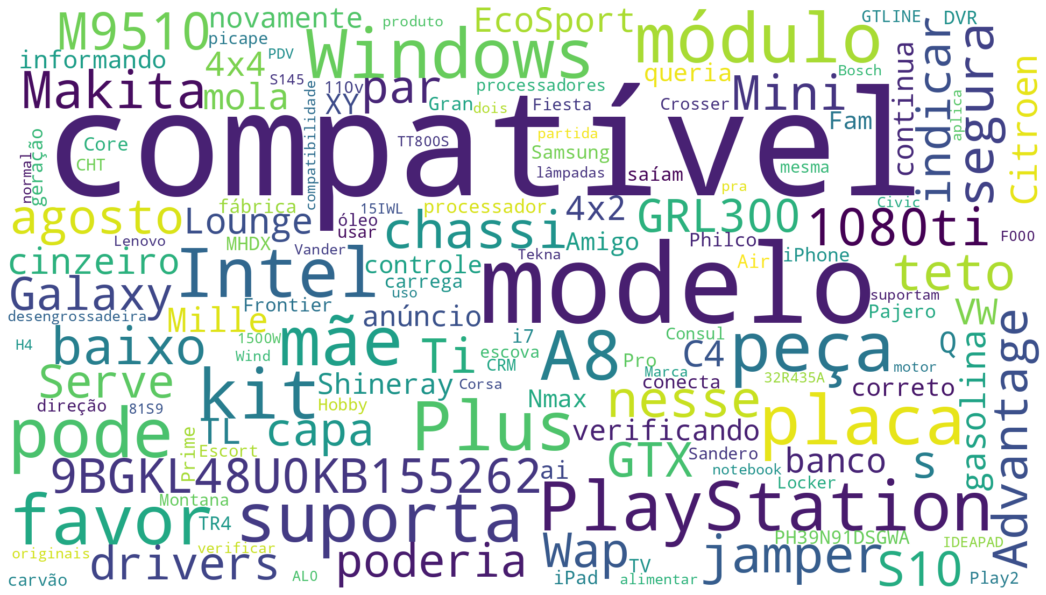
\includegraphics[width=1\linewidth]{figuras/compatible_models.png}
	\caption{Nuvem de palavras gerada a partir dos exemplos de Treino e Teste da classe \textbf{COMPATIBLE\_MODELS}, após remoção de \textit{stopwords}.}
	\label{fig:compatible_models}
\end{figure}

\clearpage % Para garantir que as imagens não irão ser mostradas na próxima Seção
\section{Considerações Finais}
Neste capítulo, uma visão geral dos resultados obtidos em cada etapa do trabalho foi apresentada. Foi feita uma análise da representatividade de cada atributo definido como classe em relação ao número de subcategorias de produtos do Mercado Livre em que esse atributo pode ser utilizado. Além disso, foi realizada uma estimativa da quantidade de dados coletados de cada fonte. Uma análise em relação ao número de exemplos rotulados de cada classe e as condições que levaram ao desbalanceamento entre as classes também foi feita.

Após testes com cinco configurações de modelos classificadores e duas configurações de base de dados, foi possível escolher o modelo HF2 como o melhor algoritmo de classificação. O modelo mostrou ser especialista em algumas classes na configuração de base de dados original, que se aproxima mais do problema real. Em seguida, o modelo foi aplicado sobre a base de dados aglutinada e melhorou substancialmente suas métricas de avaliação, o que indica a eficiência desse procedimento na recategorização de perguntas que poderiam pertencer a mais de uma classe. O modelo RASA3 também apresentou um resultado positivo: foi o segundo melhor modelo de acordo com as métricas de avaliação e se mostrou mais generalista.

A partir dos resultados obtidos, foi possível concluir que o método apresentado é eficaz em classificar corretamente variados tipos de perguntas. No entanto, algumas classes são frequentemente confundidas em todos os modelos testados por falta de conhecimento de mundo. Por isso, avaliações de outras metodologias deveriam ser feitas caso haja interesse em classificar essas classes de forma satisfatória.

% Avaliação dos Classificadores: todas as matrizes de confusão, assim como as tabelas de resultado das duas planilhas. Primeiro apresentar BERT-40classes, depois DIET-40classes, e depois os dois juntos no experimento com 28 classes.

% A comparação RASA1 vs. RASA3 é interessante, uma vez que a única diferença entre as duas pipelines é a etapa de pré-processamento dos dados. Salientar o CountVectorsFeaturizer que se saiu superior. Porém, não me parece natural apresentar esse resultado antes da Avaliação dos Classificadores em si.

% Assim como na página 59 do TCC do Oscar, talvez fazer um ranking das 5 classes mais acertadas pelo HF em porcentagem (para desconsiderar o desbalanceamento)

% Tentar investigar o porquê de classes que tiveram desempenho falho, mesmo no melhor modelo, falharam. Talvez com nuvens de palavras.
% COMPATIBLE_BRANDS: apenas 1 ou outro VERDADEIROS POSITIVOS foram encontrados em todos os testes. É a classe que foi menos acertada (ver qual métrica é essa). Provavelmente foi confundida com COMPATIBLE_MODELS. Comparar as palavras da nuvem de palavras de cada uma para perceber que as palavras são as mesmas e falta conhecimento de mundo. Apresentar como solução para isso o uso do grafo de conhecimento do Mercado Livre do que são MARCAS e do que são MODELOS ou usar modelos com muito mais parâmetros (como as LLMs) sempre que uma pergunta for classificada como COMPATIBLE_X.

% Mostrar que, nas classes que o BERT se sai bem, ele acerta MAIS do que o RASA. No entanto, nas classes em que ambos os modelos se saem mal, o RASA acerta 1 ou outro exemplo. O BERT pode ser especialista, o RASA generalista.


